\documentclass[11pt,a4paper]{article}
\usepackage[utf8]{inputenc}
\usepackage[T1]{fontenc}
\usepackage{lmodern}
\usepackage[margin=2.4cm]{geometry}
\usepackage{amsmath}
\usepackage{graphicx}
\usepackage{booktabs}
\usepackage{microtype}
\usepackage[font=small,labelfont=bf]{caption}
\usepackage{xcolor}
\usepackage[colorlinks=true,linkcolor=blue!50!black,urlcolor=blue!50!black]{hyperref}
\usepackage{float}

\renewcommand{\figurename}{Figura}
\renewcommand{\tablename}{Tabela}
\graphicspath{{../results/k5/figs/}}
\setlength{\parskip}{0.55em}
\setlength{\parindent}{0pt}

\title{\textbf{Projeto 4: Previsão de temperatura com LSTM}}
\author{Aline Breda Kuster (RA: 168495) \\ \small Introdução às Redes Neurais Artificiais, UNIFESP \\
\small Repositório: \textcolor{red}{(colocar o link do GitHub)}}
\date{}

\begin{document}
\maketitle
\vspace{-2.5em}

\section{Objetivo e dados}

O objetivo é treinar uma rede recorrente para prever o valor de uma série temporal no futuro. Escolhi a tarefa de
previsão: a rede recebe a temperatura mínima dos últimos $W$ dias, até o dia $t$, e prevê a temperatura do dia
$t+k$, com $k=5$, ou seja, cinco dias à frente.

A série usada é a temperatura mínima diária de Melbourne, na Austrália, de 1981 a 1990, com 3\,650 dias. Ela tem um
ciclo anual bem marcado (verões perto de 15\,°C e invernos perto de 7\,°C) e bastante variação de um dia para o outro.

Os dados foram divididos em ordem cronológica, pela data do dia previsto: 1981 a 1986 para treino, 1987 e 1988 para
validação e 1989 e 1990 para teste (Figura~\ref{fig:serie}). Em série temporal a divisão não pode ser aleatória,
porque o modelo estaria treinando com dias vizinhos aos que vai prever e o resultado ficaria otimista. As
temperaturas foram normalizadas com a média e o desvio padrão do período de treino.

\begin{figure}[H]
\centering
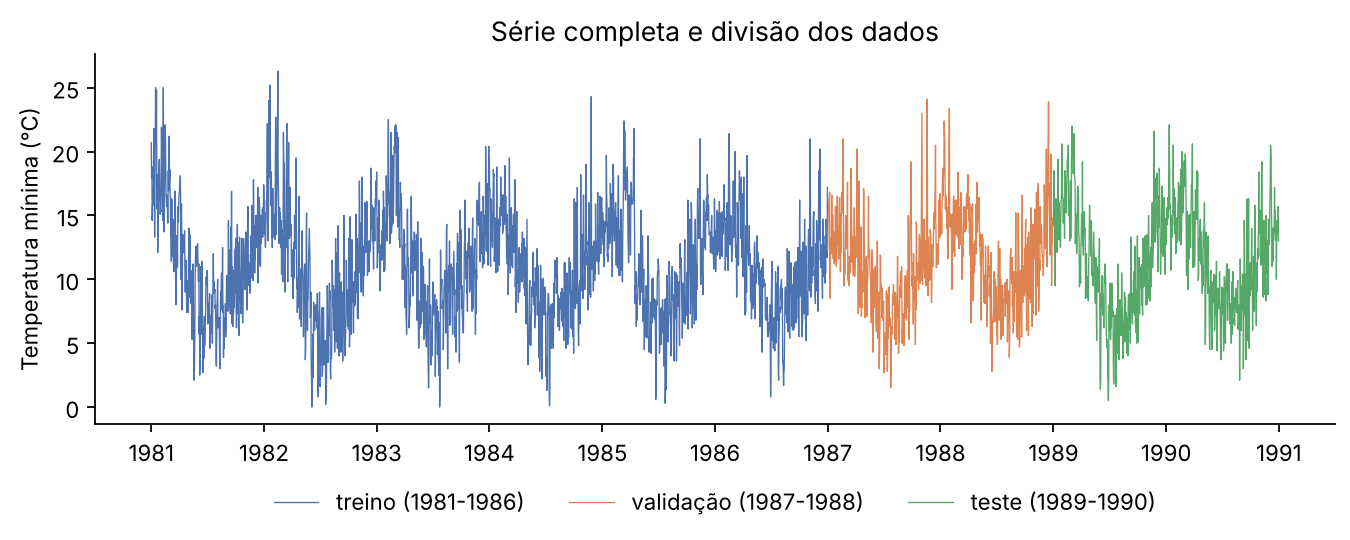
\includegraphics[width=\linewidth]{serie.png}
\caption{Temperatura mínima diária e a divisão em treino, validação e teste.}
\label{fig:serie}
\end{figure}

Cada exemplo é uma janela com os $W$ dias anteriores e o valor do dia $t+5$ como alvo. Com uma janela de 60 dias, por
exemplo, ficam 2\,126 janelas de treino, 730 de validação e 730 de teste.

\section{Modelo}

O modelo é uma LSTM, uma rede recorrente que lê a janela um dia de cada vez. A cada passo ela combina a temperatura do
dia com um estado interno que resume os dias anteriores, e suas portas decidem o que guardar e o que esquecer desse
estado. Depois de ler o último dia da janela, o estado final passa por uma camada linear que devolve um único número:
a temperatura prevista para $t+5$.

O treino usa o erro quadrático médio (MSE) como função de custo, o otimizador Adam, lotes de 64 janelas e
\emph{dropout} de 0,2 entre camadas quando há mais de uma. O treino para quando a perda de validação passa 10 épocas
sem melhorar, e os pesos da melhor época são mantidos.

\section{Ajuste dos hiperparâmetros}

Fiz uma busca em grade com quatro hiperparâmetros: o tamanho da janela (14, 30 ou 60 dias), o número de neurônios da
LSTM (32 ou 64), o número de camadas (1 ou 2) e a taxa de aprendizado (0,001 ou 0,005). São 24 combinações, todas
treinadas e comparadas pelo RMSE no conjunto de validação (Figura~\ref{fig:busca}).

\begin{figure}[H]
\centering
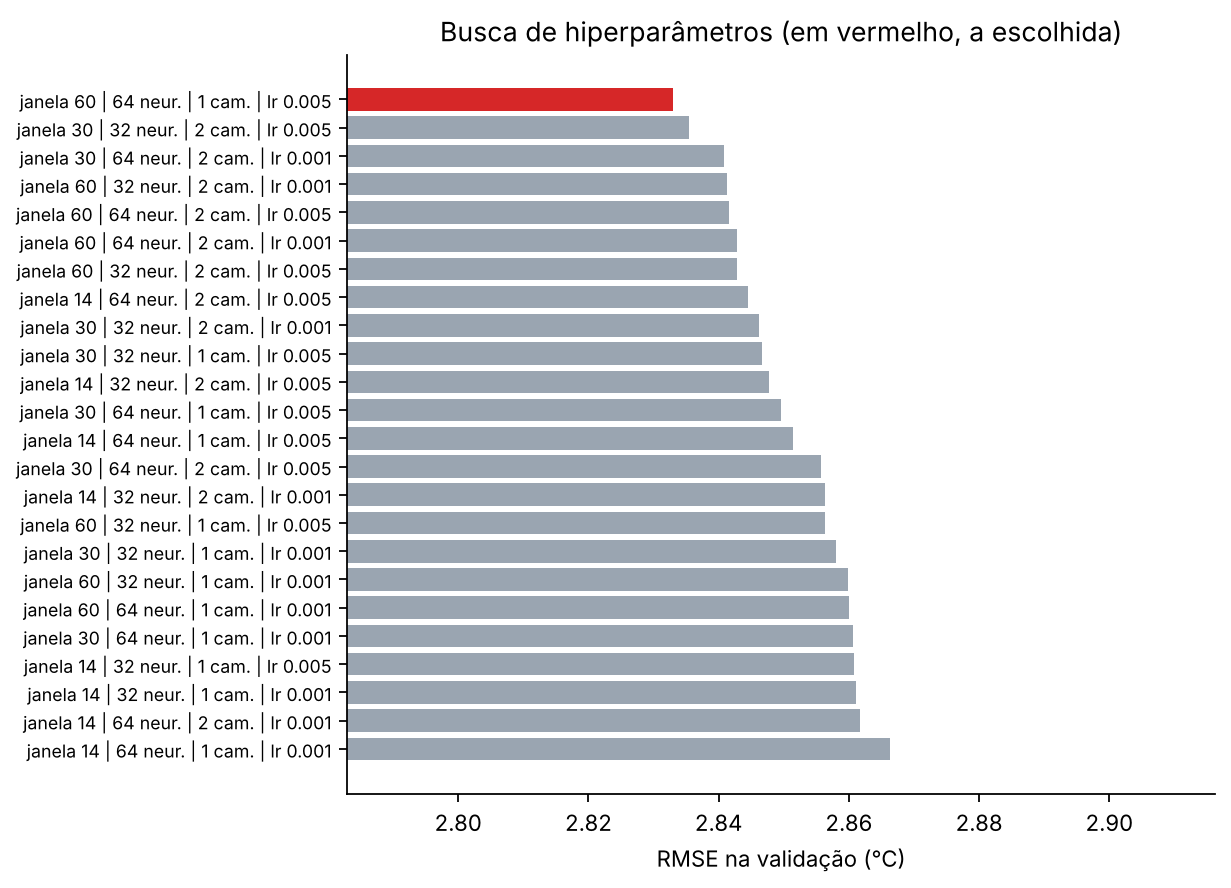
\includegraphics[width=0.78\linewidth]{busca.png}
\caption{RMSE de validação das 24 combinações (janela $|$ neurônios $|$ camadas $|$ taxa de aprendizado).}
\label{fig:busca}
\end{figure}

A melhor combinação foi a janela de 60 dias, 64 neurônios, 1 camada e taxa de aprendizado de 0,005, com RMSE de
validação de 2,83\,°C. O modelo tem 17\,217 parâmetros. As diferenças entre as combinações foram pequenas: a pior
ficou com 2,87\,°C, só 0,03\,°C acima. Ainda assim há um padrão: as redes de 2 camadas aparecem mais no topo da lista, e as
de 1 camada com taxa de 0,001 ficam no fim, junto com a maior parte das janelas de 14 dias. Uma janela maior dá mais
contexto sobre a tendência da estação, mas o ganho é pequeno, porque o que mais pesa na previsão a 5 dias é o nível
recente da temperatura, que todas as janelas já contêm.

\section{Curva de aprendizagem}

A Figura~\ref{fig:curva} mostra o RMSE de treino e de validação a cada época do modelo escolhido. A época 0 é o erro
antes do treino, com pesos aleatórios.

\begin{figure}[H]
\centering
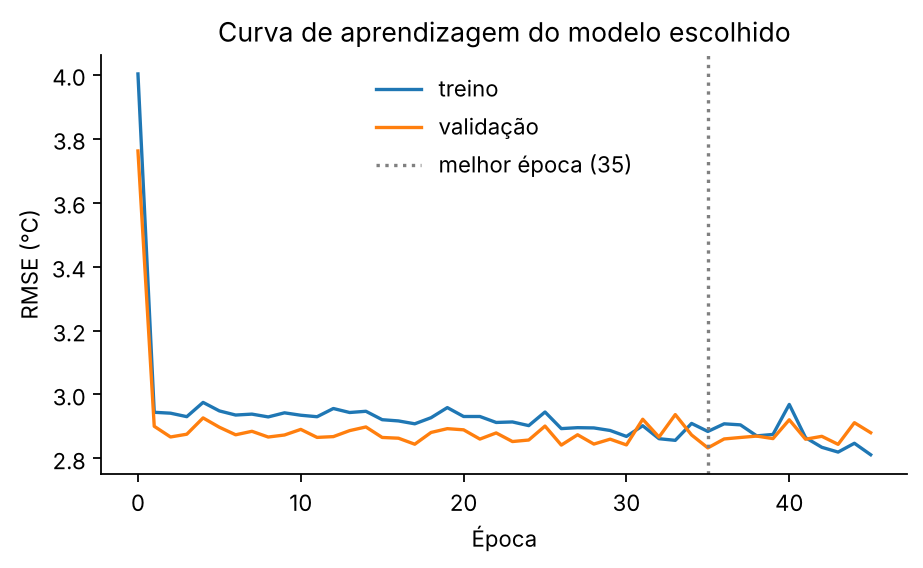
\includegraphics[width=0.7\linewidth]{curva_aprendizagem.png}
\caption{RMSE de treino e de validação por época do modelo escolhido. A linha pontilhada marca a época mantida.}
\label{fig:curva}
\end{figure}

Quase todo o aprendizado acontece na primeira época, em que o erro cai de cerca de 4\,°C para 2,9\,°C. Nesse começo a
rede aprende o principal, que é acompanhar o nível da temperatura e o ciclo das estações. Depois disso o erro cai
devagar até a época 35, que teve o menor erro de validação (2,83\,°C). O treino parou na época 45, depois de 10 épocas
sem melhora. As curvas de treino e validação ficam próximas o tempo todo, então não houve sobreajuste. As oscilações
vêm da taxa de aprendizado mais alta, que faz os pesos se moverem mais a cada passo.

\section{Avaliação no teste}

O modelo foi avaliado uma única vez no teste (1989 e 1990). Para ter uma referência, comparei com a
\textbf{persistência}, que prevê que daqui a 5 dias a temperatura será igual à de hoje. Usei três métricas, todas em
graus: o MAE (erro absoluto médio), o RMSE (raiz do erro quadrático médio, que pesa mais os erros grandes) e o $R^2$,
que indica quanto da variação da temperatura o modelo explica (1 seria uma previsão perfeita).

\begin{table}[H]
\centering
\caption{Métricas no conjunto de teste (1989-1990).}
\label{tab:metricas}
\begin{tabular}{lccc}
\toprule
Modelo & MAE (°C) & RMSE (°C) & $R^2$\\
\midrule
LSTM & 2,09 & 2,69 & 0,57\\
Persistência & 2,81 & 3,49 & 0,28\\
\bottomrule
\end{tabular}
\end{table}

A LSTM erra em média 2,1\,°C e tem RMSE 23\% menor que a persistência. O erro no teste (2,69\,°C) ficou até um pouco
menor que na validação (2,83\,°C), então o modelo generalizou bem para anos que não viu.

\begin{figure}[H]
\centering
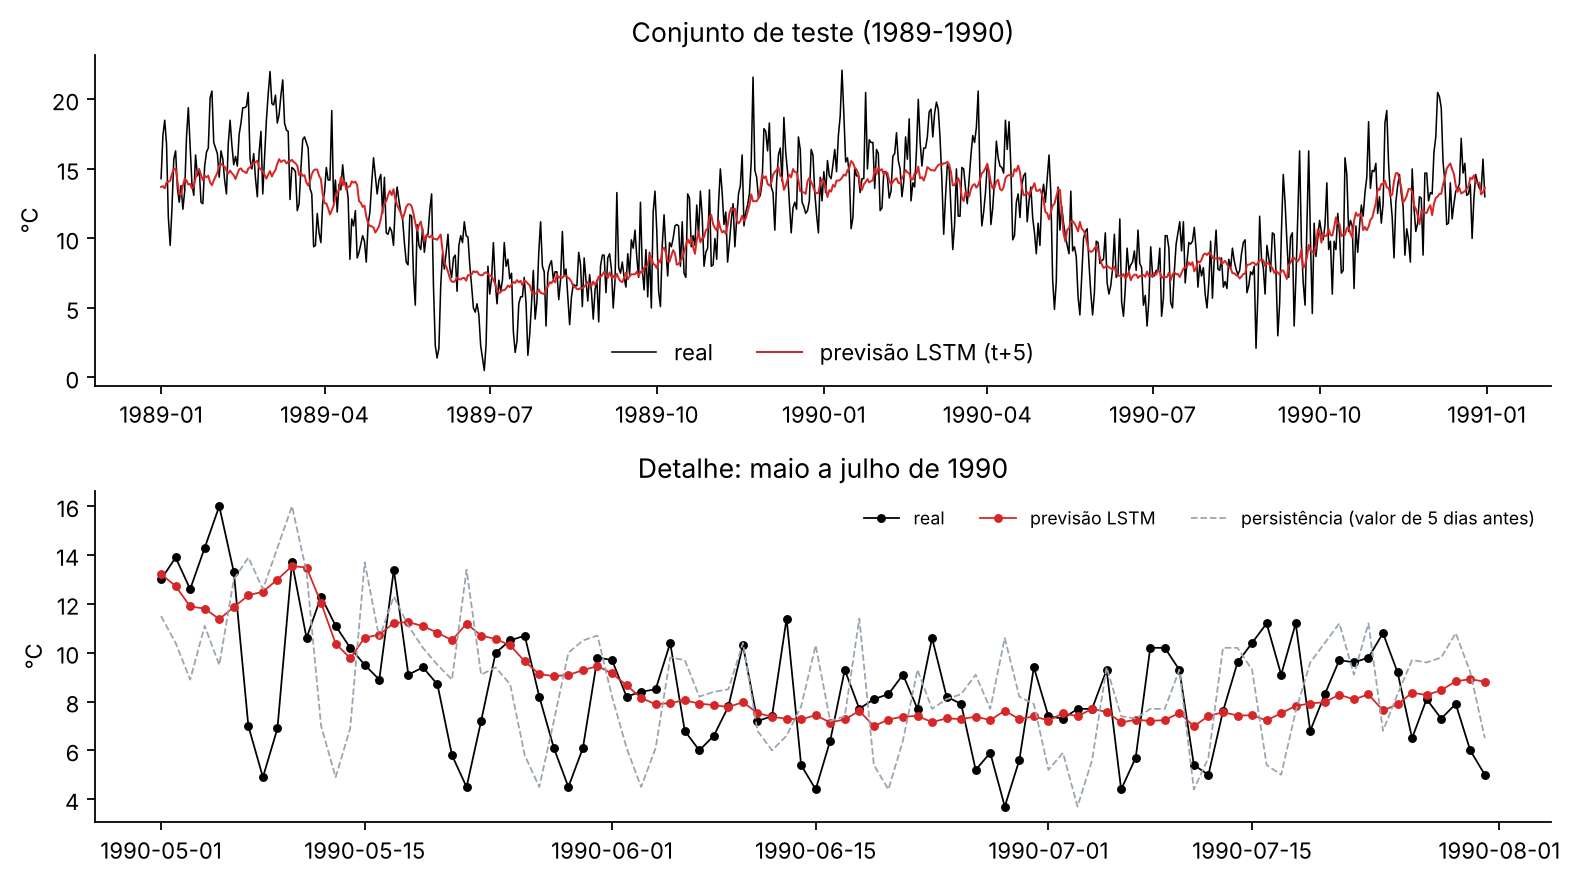
\includegraphics[width=\linewidth]{previsao_teste.png}
\caption{Temperatura real e prevista no teste. Embaixo, um trecho de três meses com a persistência para comparação.}
\label{fig:prev}
\end{figure}

A Figura~\ref{fig:prev} mostra o comportamento do modelo. A previsão acompanha bem o ciclo anual e as mudanças de
tendência, mas é mais suave que a série real: os picos de calor e as noites muito frias não são previstos. Isso é
esperado, porque essas variações bruscas dependem do tempo de cada dia, que não pode ser antecipado só com as
temperaturas passadas. A persistência, no trecho de baixo, copia essas oscilações com 5 dias de atraso e por isso erra
mais. A LSTM aprendeu a não seguir o ruído e a ficar perto do valor mais provável.

\subsection*{Efeito da distância da previsão}

Para ver como a distância $k$ afeta o resultado, repeti todo o processo para $k=1$, ou seja, prever a temperatura do
dia seguinte, com a mesma busca de 24 combinações escolhida pela validação (Tabela~\ref{tab:k}).

\begin{table}[H]
\centering
\caption{Resultado no teste para previsão de 1 e de 5 dias à frente. Cada $k$ teve sua própria busca de hiperparâmetros.}
\label{tab:k}
\begin{tabular}{ccccc}
\toprule
$k$ & Melhor combinação & RMSE LSTM (°C) & RMSE persistência (°C) & $R^2$ LSTM\\
\midrule
1 & janela 60, 32 neur., 2 camadas, lr 0,005 & 2,21 & 2,48 & 0,71\\
5 & janela 60, 64 neur., 1 camada, lr 0,005 & 2,69 & 3,49 & 0,57\\
\bottomrule
\end{tabular}
\end{table}

Prever o dia seguinte é mais fácil: o erro cai para 2,21\,°C e o $R^2$ sobe para 0,71. A persistência também melhora
bastante com $k=1$, porque a temperatura de amanhã costuma ser parecida com a de hoje, e por isso a vantagem da LSTM
fica menor, de 11\%. Com $k=5$ a persistência piora muito mais que a LSTM, e a vantagem sobe para 23\%: quanto mais
longe a previsão, mais vale ter um modelo que aprendeu a estação e a tendência em vez de só copiar o valor de hoje. A
melhor topologia também mudou de um $k$ para o outro, o que mostra que os hiperparâmetros precisam ser ajustados para
cada tarefa.

\section{Considerações finais}

A LSTM conseguiu prever a temperatura mínima com 5 dias de antecedência com erro médio de 2,1\,°C, bem melhor que a
persistência. Com 1 dia de antecedência o erro é menor, mas a vantagem sobre a persistência também diminui. Na busca, a janela de 60 dias com uma camada de 64 neurônios foi a melhor, mas as combinações ficaram
muito próximas, sinal de que o limite está na própria série: o modelo capta a estação e a tendência recente, e o que
sobra é a variação de curto prazo do tempo, que a temperatura passada sozinha não explica. Para melhorar, seria
preciso acrescentar outras variáveis, como umidade, pressão e vento.

\end{document}
